\thispagestyle{fancy}

\chapter{Untersuchung der optischen Polarisation an AlGaN MQWs mit Photolumineszenzspektroskopie}
\label{chap:pol}
\section{Einleitung}
Um die Polarisation und den Kreuzungspunkt der Simulationen von Christoph Reich experimentell zu \"uberpr\"ufen, wurden die Polarisation von zwei Probenserien mit Hilfe von Photolumineszenz-Spektroskopie untersucht. Die untersuchten Probenserien unterteilen sich in eine QW-Dicken-Variation (Serie A) und einer Serie mit Variation des Al-Gehalts (Serie B) in den QWs. 
Die Proben wurde alle bei Raumtemperatur (300K) untersucht und die Emission wurde aus der Kante der Probe gemessen um das Verhältnis zwischen TE- und TM-polarisertem Licht zu bestimmen. Weil es m\"oglicherweise Auswirkungen des ELO auf die Polarisation gibt, wurde der Einfluss des ELO mit untersucht. 

\section{Variation des Al-Gehalts in den QWs}

Die Untersuchung der Al-Variations Serie, dient dem Zweck, anhand eines variierenden Al-Gehalts in den QWs und einem festen Al-Gehalt in der Barriere den \"Ubergang von TE zu TM (siehe Abb. \ref{fig:simuchr} in Kapitel \ref{chap:polgrund}) bei fester QW-Dicke experimentell zu \"uberpr\"ufen. Dazu wurden vier Proben auf ELO-AlN gewachsen, mit einer darauf folgenden AlN(100\%) Buffer-Schicht. Auf die Buffer-Schicht folgt zuletzt die aktiven Zone, mit einem zwischen der ersten und letzten undotierten AlN-Barriere eingebetteten dreifach $Al_{x}Ga_{1-x}N$ QWs mit einer Dicke von $1,5nm$ und dazwischen AlN-Barrieren einer Dicke von $5nm$. Der Aluminium-Gehalt der QWs wurde variiert mit x= 60 \%, 68 \%, 73 \%, 81 \%. 
Der Einfluss des unterschiedlichen Al-Gehalts auf die Emissionsenergie ist in Abb. [\ref{fig:alvariationSpektrum}] zu erkennen. Die kleinste Wellenl\"ange hat Probe A:4 mit einem Al-Gehalt von $81\%$, die theoretisch ausreicht um im Vergleich mit den anderen Proben zumindest einen Abfall des Polarisationgrades der TE-Polarisation zu erkennen.
%
\begin{figure}[htb]
  \centering
  \begin{minipage}[t]{0.49\textwidth}
    \centering
    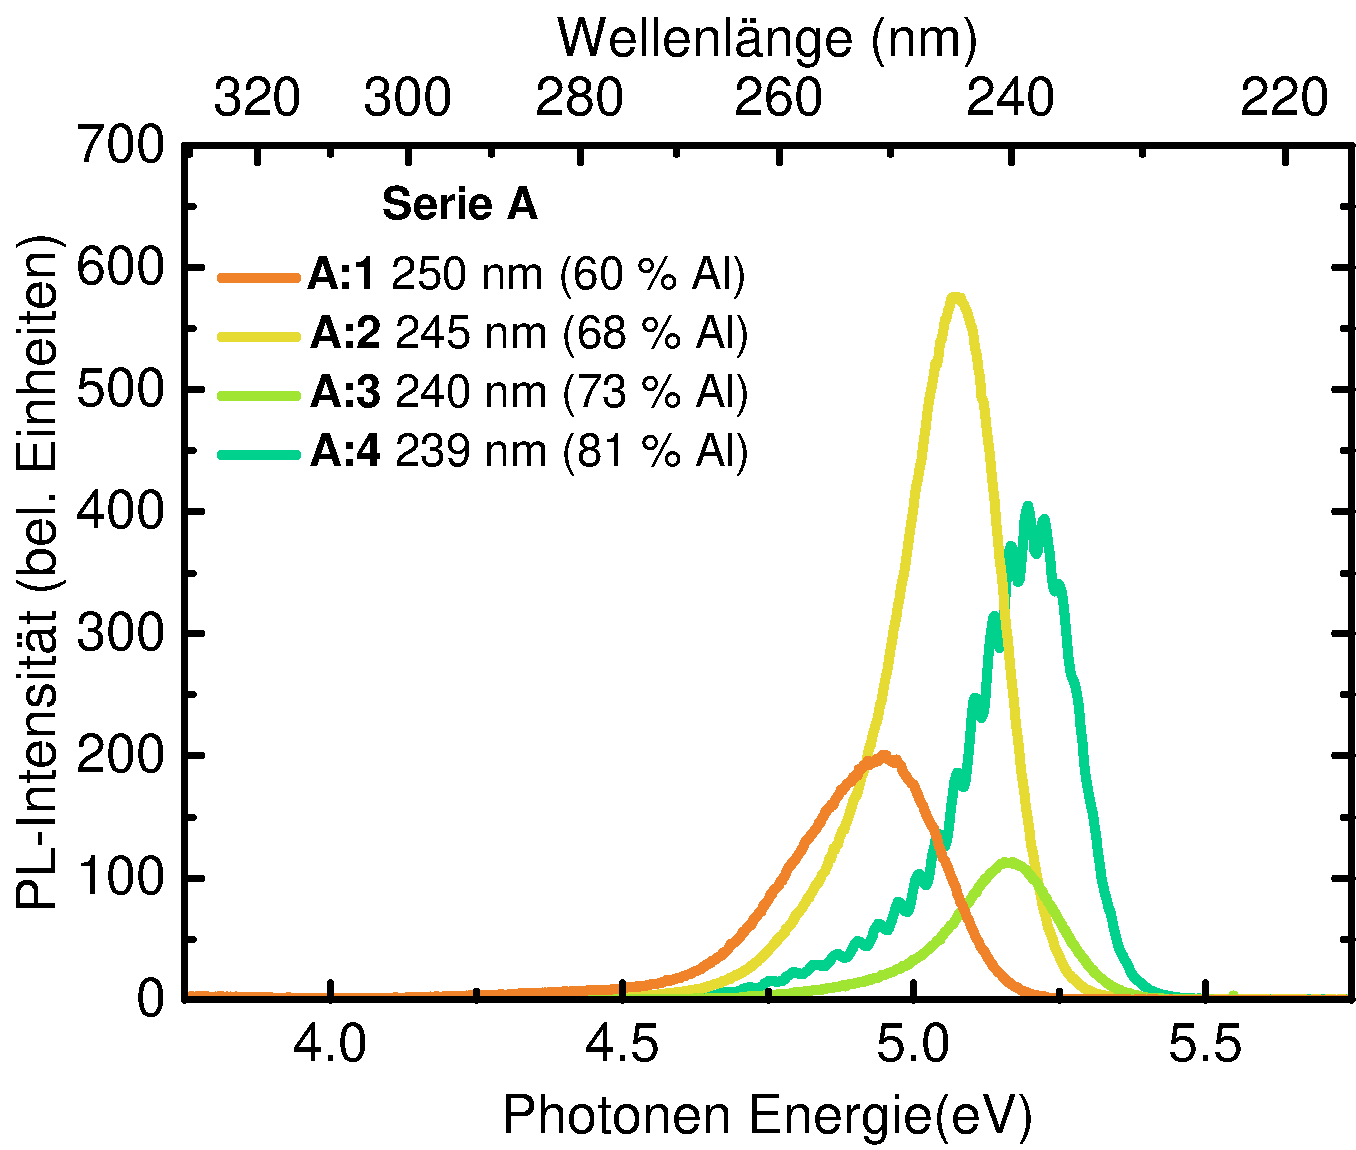
\includegraphics[width=\textwidth]{Bilder/spektrenAlvariation.pdf}
    \caption{PL-Spektren der Serie A. Die Emission verschiebt sich mit steigendem Al-Gehalt in den QWs hin zu kleineren Wellenl\"angen durch die steigende Bandl\"uckenenergie. }
    \label{fig:alvariationSpektrum}
  \end{minipage}
	\hfill
  \begin{minipage}[t]{0.49\textwidth}
    \centering
    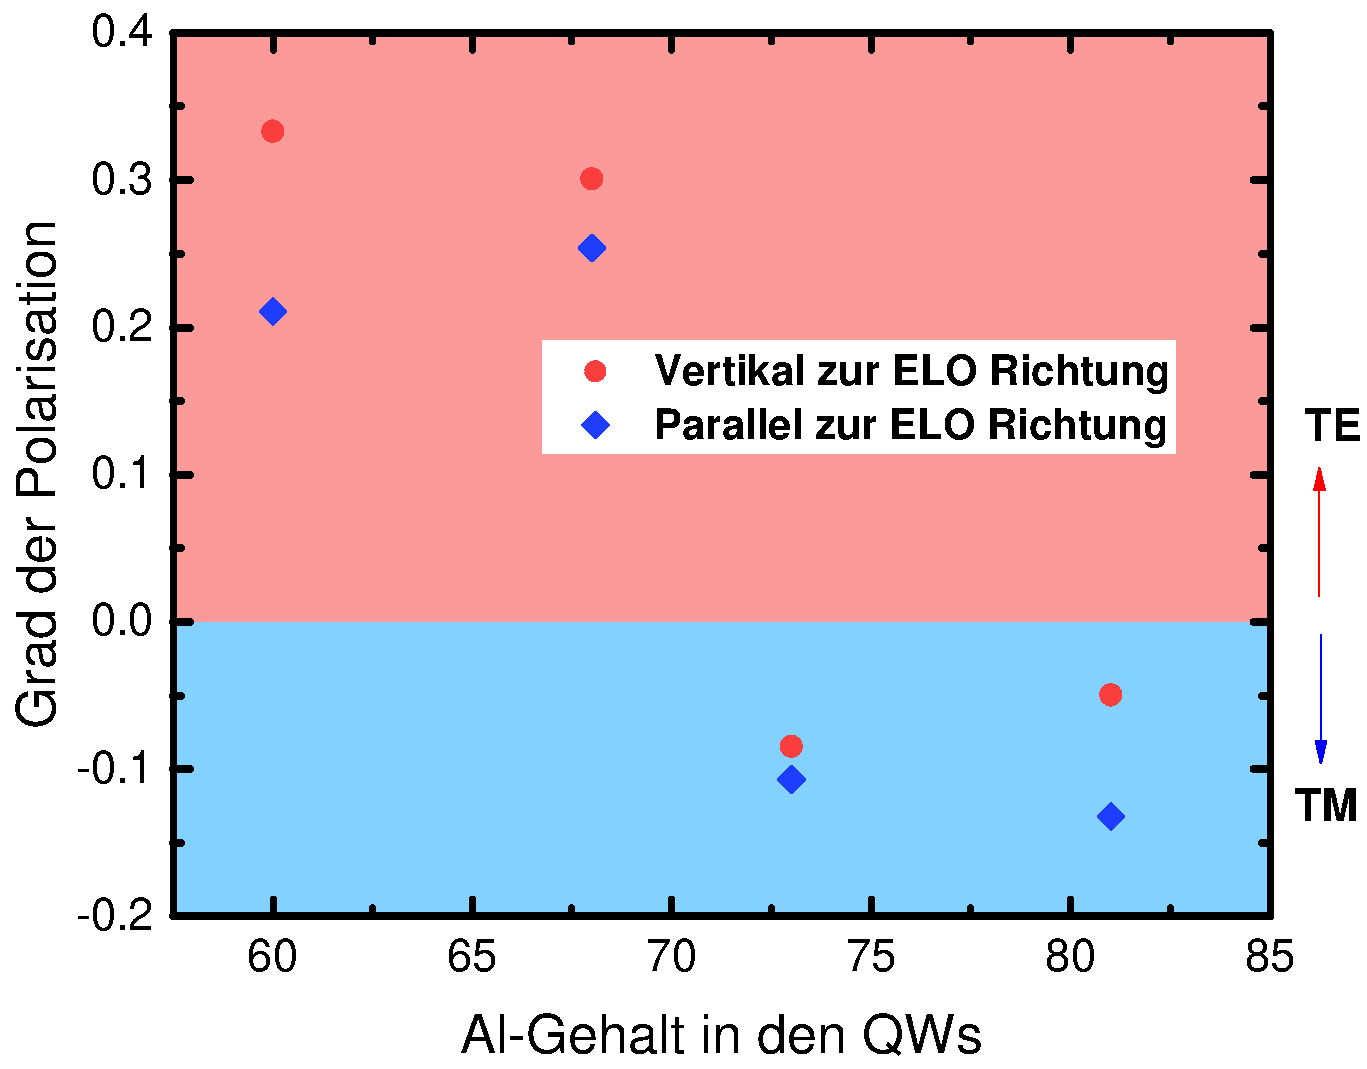
\includegraphics[width=\linewidth]{Bilder/polarisationAlvariation.pdf}
    \caption{Ergebnisse der Polarisationsmessungen an Serie A mit den Polarisationsgraden abh\"angig vom Al-Gehalt des QW und zus\"atzlich mit den Messwerten in Abh\"angigkeit der ELO-Richtung. }
    \label{fig:alvariationPolarisation}
  \end{minipage}
\end{figure}
%
Dazu wurden Proben vertikal und horizontal zur ELO-Richtung positioniert und gemessen. Abbildung [\ref{fig:alvariationPolarisation}] zeigt die Ergebnisse der Polarisationsmessungen. So zeigen die Proben A:1 und A:2 mit einem Al-Gehalt von $60\%$ und $68\%$ TE-Polarisation. Der Grad der Polarisation ist zus\"atzlich noch abh\"angig von der Positionierung der ELO-Streifen. So haben die Proben A:1 und A:2 vertikal zur ELO-Richtung Polarisationsgrade von $\rho = 0,33$ und $\rho = 0,30$ und parallel zur ELO-Richtung deutlich geringe Polarisationsgrade mit $\rho = 0,22$ und $\rho = 0,25$. Die Proben A:3 und A:4 mit $73\%$ und $81\%$ Al-Gehalt weisen TM-Polarisation auf mit Polarisationsgraden von $\rho = -0,09$ und $\rho = -0,05$ vertikal zur ELO-Richtung und $\rho = -0,11$ und $\rho = -0,14$ parallel zur ELO-Richtung. Es zeigt sich demzufolge, dass die Polarisation sich mit steigendem Al-Gehalt von TE- hin zu TM-Polarisation \"andert durch die Neuordnung der Valenzb\"ander. Der Wechsel findet bei einer Wellenl\"ange von ca. $240nm$ statt und ist in guter \"Ubereinstimmung mit den Simulation (siehe Abb. [\ref{fig:simuchr}]). \"Uberdies ist eine Abh\"angigkeit der Ausrichtung der ELO-Streifen zu beobachten. M\"ogliche Erkl\"arungen w\"aren, dass es durch Brechungsindexwechsel vom Freiraum des ELO zum Kristall, es zu Reflektion des emittierten Lichtes und damit zu Interferenzerscheinungen kommt oder das ELO beeinflusst die Verzerrung im Kristall so, dass die f\"ur die Simulation angenommene biaxiale Verzerrung nicht mehr zutrifft. 

\section{Variation der QW-Dicke}

Die Untersuchung der QW-Dicken Variations Serie, dient dem Zweck, anhand der variierenden QW-Dicke bei einem festen Al-Gehalt in QW und Barriere die Änderung in der Polarisation(siehe Abb. \ref{fig:simu1chr} in Kapitel \ref{chap:polgrund}) experimentell zu \"uberpr\"ufen. Dazu wurden vier Proben auf ELO-AlN gewachsen, mit einer darauf folgenden AlN(100\%) Buffer-Schicht. Auf die Buffer-Schicht folgt zuletzt die aktiven Zone, mit einem zwischen der ersten und letzten undotierten AlN-Barriere eingebetteten dreifach $Al_{0.6}Ga_{0.4}N$ QWs und dazwischen $Al_{0.81}Ga_{0.19}N$-Barrieren einer Dicke von $5nm$. 
Der Einfluss des unterschiedlichen QW-Dicke auf die Emissionsenergie ist in Abb. [\ref{fig:qwvariationSpektrum}] zu erkennen. Mit steigender QW-Dicke sinkt die Emissionsenergie und steigt die Wellenl\"ange aufgrund des QCSE und Confinements. Die Emission der Barriere ist mit steigender Dicke besser erkennbar. 
%
\begin{figure}[htb]
  \centering
  \begin{minipage}[t]{0.49\textwidth}
    \centering
    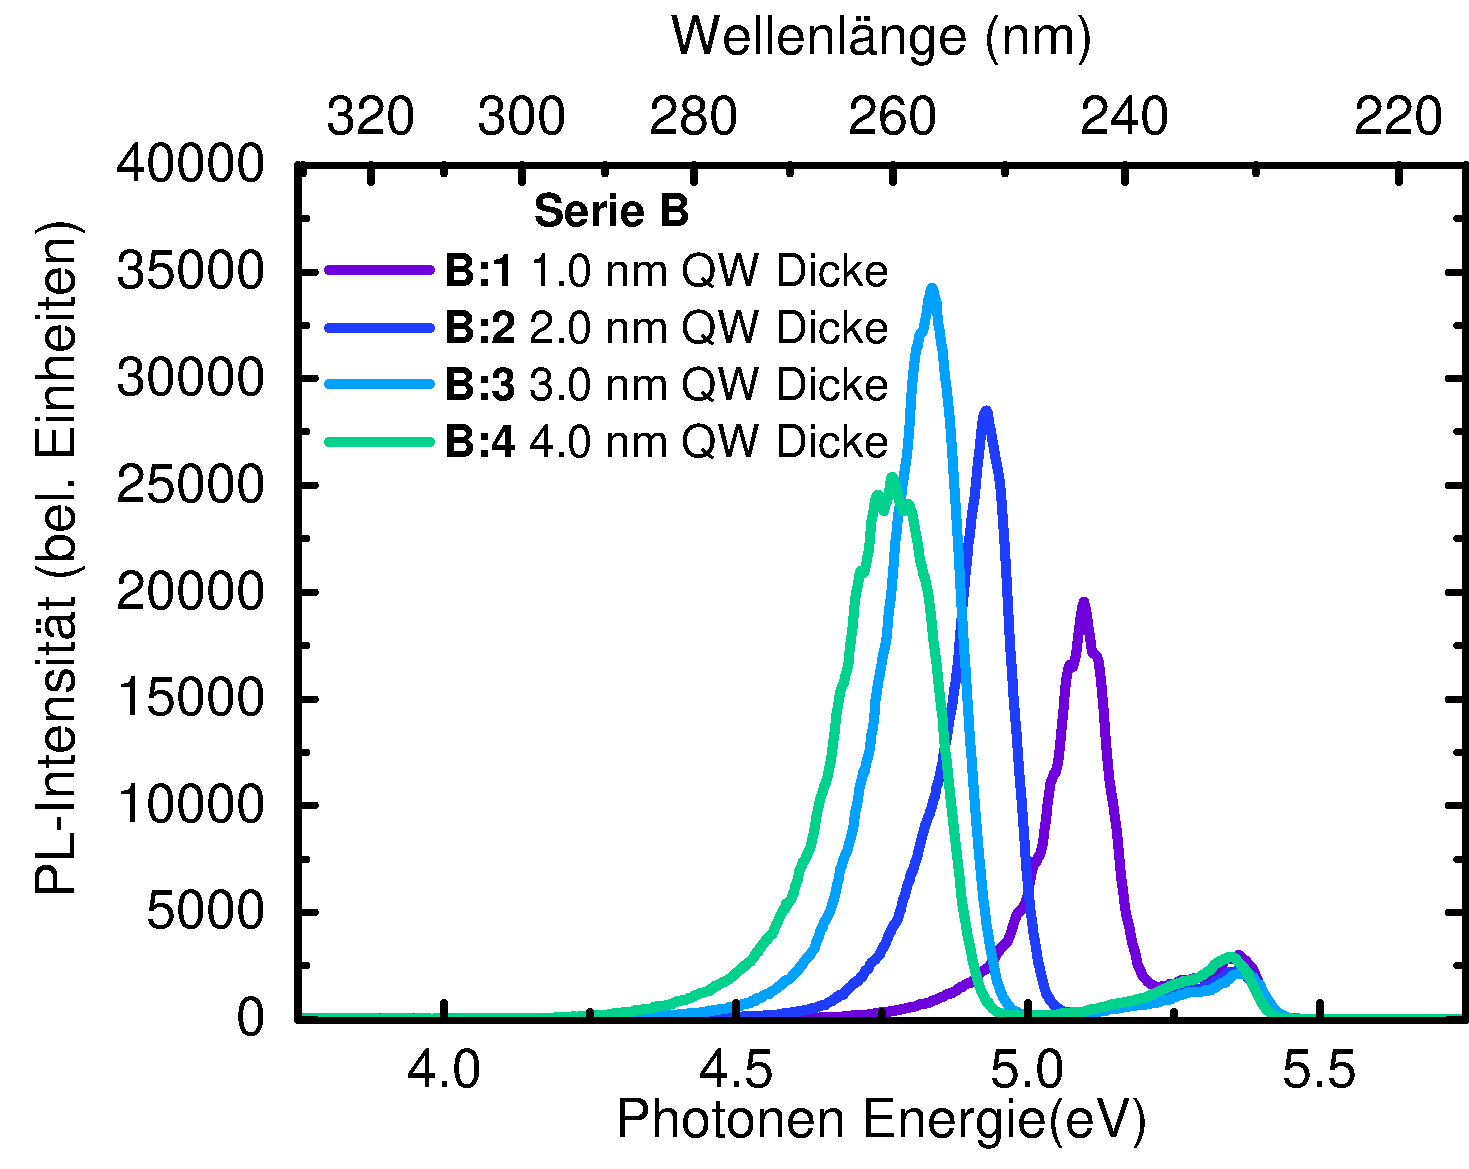
\includegraphics[width=\textwidth]{Bilder/spektrenQWvariation.pdf}
    \caption{PL-Spektren der Serie B. Die Emission verschiebt sich mit steigender QW-Dicke hin zu gr\"oßeren Wellenl\"angen durch den QCSE und Confinement.  }
    \label{fig:qwvariationSpektrum}
  \end{minipage}
	\hfill
  \begin{minipage}[t]{0.49\textwidth}
    \centering
    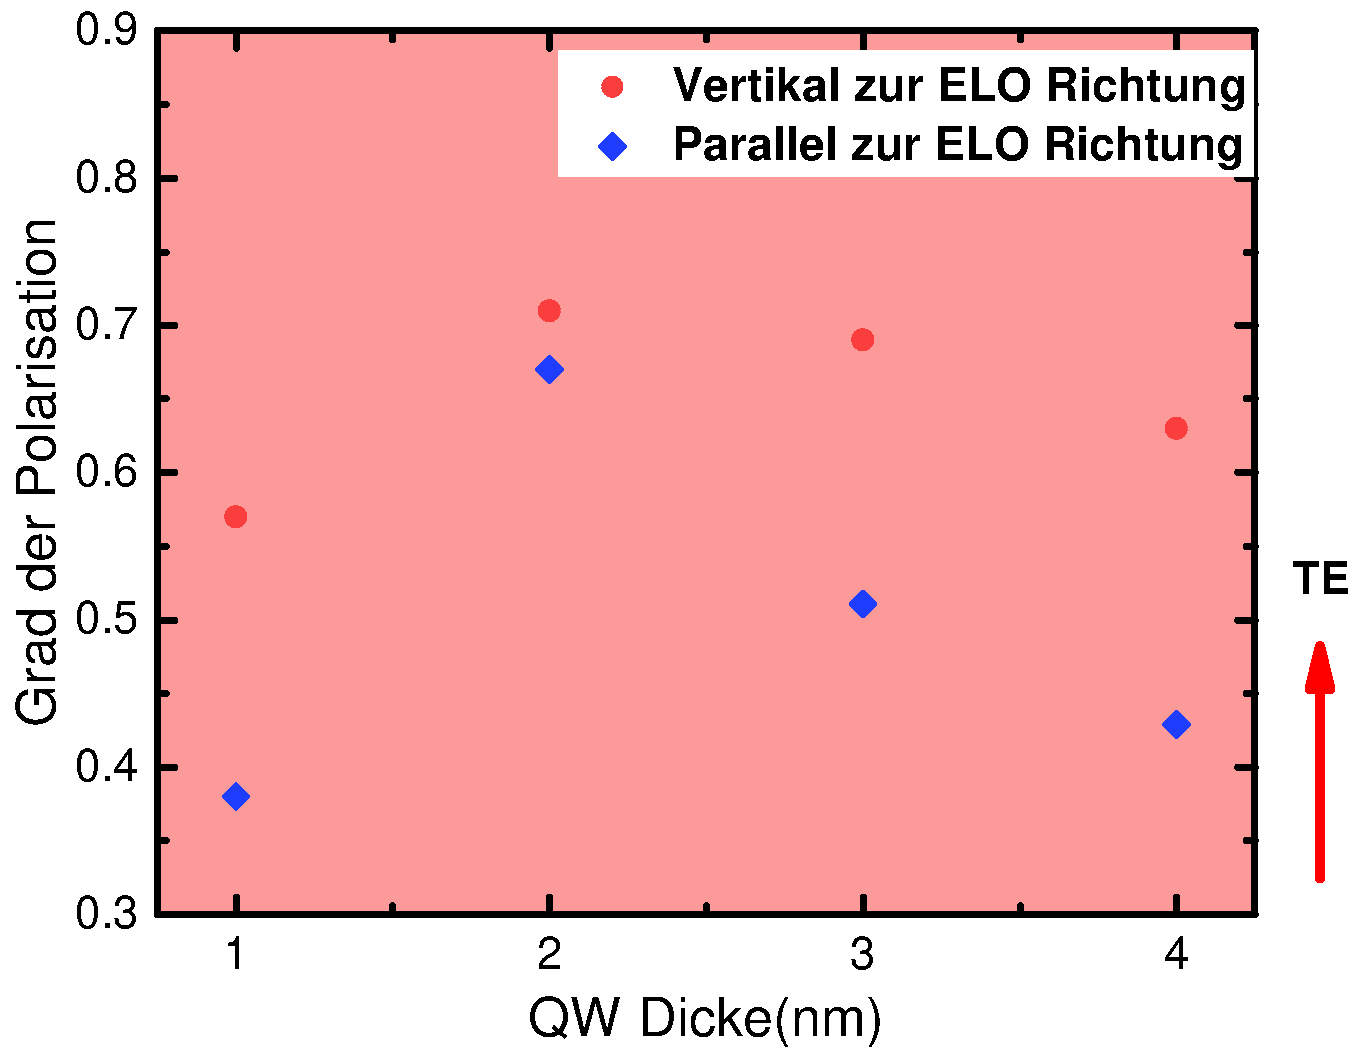
\includegraphics[width=\linewidth]{Bilder/polarisationDickenvariation.pdf}
    \caption{PL-Spektren der Serie B. Die Emission verschiebt sich mit steigendem Al-Gehalt in den QWs hin zu kleineren Wellenl\"angen durch die steigende Bandl\"uckenenergie. }
    \label{fig:qwvariationPolarisation}
  \end{minipage}
\end{figure}
%
die Ergebnisse der Polarisationsmessung zeigen eine eindeutig dominante TE-Polarisation die auch abh\"angig von der ELO-Richtung ist. Die Probe B:2 zeigt die h\"ochste TM-Polarisation mit einem Polarisationsgrad von $\rho=+0,72$ vertikal zur ELO-Richtung. Es zeigt sich, wie in der Simulation
in Abb. \ref{fig:simu1chr} zu sehen, dass mit einem Al-Gehalt von $60$\% in den QWs, der Polarisationsgrad bei den Proben mit $1$ und $4 \thinspace nm$ QW-Dicke am niedrigsten ausf\"allt und bei $2 \thinspace nm$ am h\"chsten. Somit best\"atigt der Verlauf die Simulationen in Bezug auf den zu erwartenden Trend, wo am Rand zum Wechsel (bei $1$ und $4 \thinspace nm$) von TE zu TM der geringste Polarisationsgrad zu erwarten ist.
